%!TEX program = xelatex 
\documentclass[hyperref, UTF8
,bookmarksnumbered=true, oneside]{ctexbook}
\hypersetup{
            bookmarksnumbered=true,
            bookmarksopen=true,
            colorlinks=false, 
            pdfborder=001,   
				%menucolor=green,%uunknown
				linktocpage=true,%make the link of the content on the number of page
            linkcolor=green,
            anchorcolor=green,
            citecolor=green}
\usepackage{geometry}
\usepackage{tocbibind}
\usepackage{graphicx}
\usepackage{amsmath}
\usepackage{amsfonts}
\usepackage{amssymb}
\usepackage{bm}
\CTEXsetup[name={(,)}]{chapter}
%\CTEXsetup[number={\chinese{section}}]{section}


\newcommand{\beqt}{\begin{equation}}
\newcommand{\eeqt}{\end{equation}}
\newcommand{\beqtnt}{\begin{equation*}}
\newcommand{\eeqtnt}{\end{equation*}}

\geometry{a4paper,centering,scale=0.8}

\title{\huge{软件工程课程作业}\\ \Huge \textbf{Mathematica Input Assistant} \\\phantom{aaa} \\\Huge{设计文档}}
\author{\\ \phantom{aaa} \\\phantom{aaa} \\ \phantom{aaa}\\\\\\\huge{待定小组}\\\\ \Large{基科物理32{  }蒋文韬}\\ \Large{基科物理32{ }张思源{ }}\\ \Large{基科应用31{ }李泽清{ }} \\ \Large{基科应用31 { }傅笛{ }} }
\begin{document}\Large

\frontmatter
\maketitle

\tableofcontents

\mainmatter

\chapter{概述}

	\section{简介} % (fold)

		Mathematica是一款类似MatLab的科学计算软件,与MatLab相比扩展功能与包较少,但符号计算功能十分强大,并且绘图效果更佳,学习数学与物理方向的同学较为常用。然而,Mathematica界面十分简单,与office软件等不同,其众多功能不是展示在用户眼前的,用户需要对能够完成他们需求的函数与代码比较熟悉。对没用过的人与初学者来说与记事本看起来一样,让人无从下手。对偶尔用一用mathematica的人,常常忘记以前用过的函数的具体名称,或者需调节的一些参数的名称与取值。另外,在Mathematica自带帮助里查找想用的函数较为不便,查找函数的参数更是十分繁多,并且帮助为英文,不便英文能力较差的使用者使用。

		因此,我们想做的是一个通过GUI实现的Mathematica输入助手,可将Mathematica的函数作为一个树结构归类显示,并对每个函数类与类中的函数都有简介与示例代码供用户拷贝进Mathematica软件运行。点选某个函数后,便可看见函数的一些常见参数与参数的简单描述,并可在下拉选项框中选择可能的参数值。选择函数并设置好参数后,即可点击生成对应的Mathematica代码,可直接拷贝进入Mathematica运行。
		
	% section 简介 (end)

	\section{软件内容与功能} % (fold)

		\begin{itemize}
			\item 用户通过树形结构与函数简介能够找到想用的函数
			\item 用户可通过函数参数的简介设置参数,生成可直接拷贝进Mathematica中使用的代码
			\item 用户可自行添加自己的函数类与函数
			\item 函数类与函数的信息通过文件保存与读取
			\item 用户可通过函数名搜索函数并点击使用 
		\end{itemize}
		
	% section 软件内容 (end)

\chapter{软件结构设计}

	\section{开发环境} % (fold)
	\label{sec:}
		\begin{itemize}
			\item 开发工具:IntelliJ IDEA 14.1.5
			\item 开发语言:Java \& Java Swing
			\item 开发环境:Windows
			\item 测试环境:Windows \& JRE 1.8.0\_60
			\item 项目管理:GitHub
		\end{itemize}
	% section  (end)
	
	\section{总体架构} % (fold)
		

		\begin{figure}[!h]
			\begin{minipage}[b]{0.45\textwidth}
			\centering
			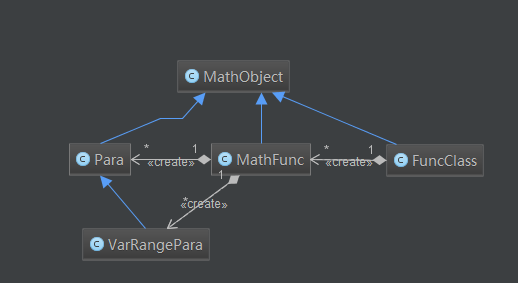
\includegraphics[width=3in]{MathPack.png}
			\caption{MathFunc Package}
			\label{pic:MathPack}
			\end{minipage}%
			\hspace{0.1\textwidth}%
			\begin{minipage}[b]{0.45\textwidth}
			\centering
			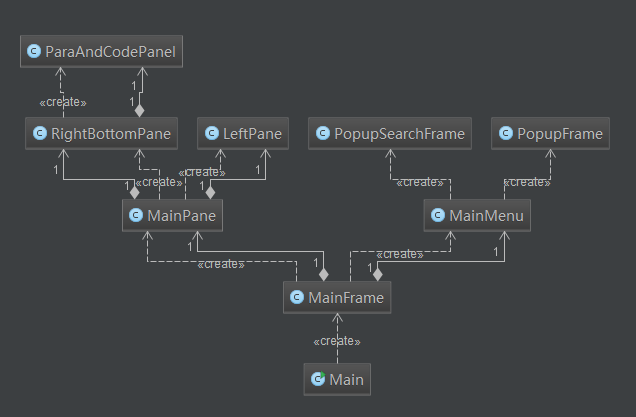
\includegraphics[width=3in]{GUIPack.png}
			\caption{GUI Package}
			\label{pic:GUIPack}
			\end{minipage}
		\end{figure}

		总体架构分为描述Mathematica函数所相关的MathFunc Package,与图形用户界面相关的GUI Package。其中MathFunc包中的类均以MathObject为父类,GUI包中的类则均为图形用户界面的不同组成部分。


		
		%\begin{figure}[!h]
		%		\centering
		%		\includegraphics[width=4in]{calc2.png}
		%		\caption{理论计算单通道计数与BBO镜架读数关系曲线图}	
		%	\label{pic:BBOAxisCalc2}
		%\end{figure}

	% section 总体架构 (end)

	\section{数学相关类} % (fold)

		\subsection{MathObject类} % (fold)
		\label{sub:mathobject}

			\begin{figure}[!h]
				\centering
				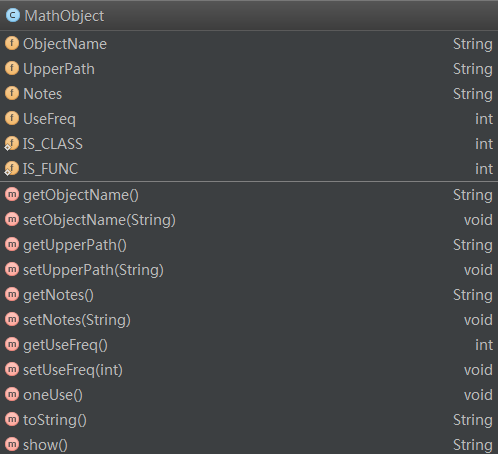
\includegraphics[width=4in]{MathObject.png}
				\caption{MathObject类成员与方法}	
				\label{pic:MathObject}
			\end{figure}

			MathObject类描述了一个抽象的数学对象,包含程序设计所需的一些成员变量,如名称,文件路径,注释等。有相应的成员方法来获取这些变量的值与更改这些变量的值。

		% subsection mathobject (end)

		\subsection{FuncClass与MathFunc类} % (fold)
		\label{sub:funcclass}
			\begin{figure}[!h]
				\begin{minipage}[b]{0.45\textwidth}
				\centering
				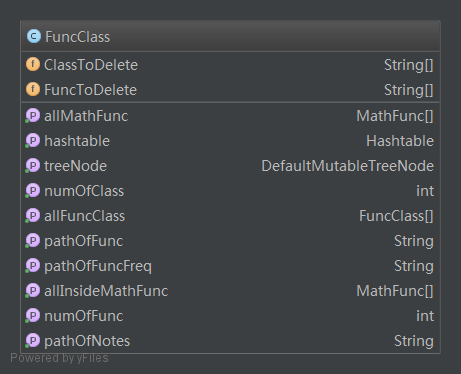
\includegraphics[width=3in]{FuncClass.png}
				\caption{FuncClass类}
				\label{pic:MathPack}
				\end{minipage}%
				\hspace{0.1\textwidth}%
				\begin{minipage}[b]{0.45\textwidth}
				\centering
				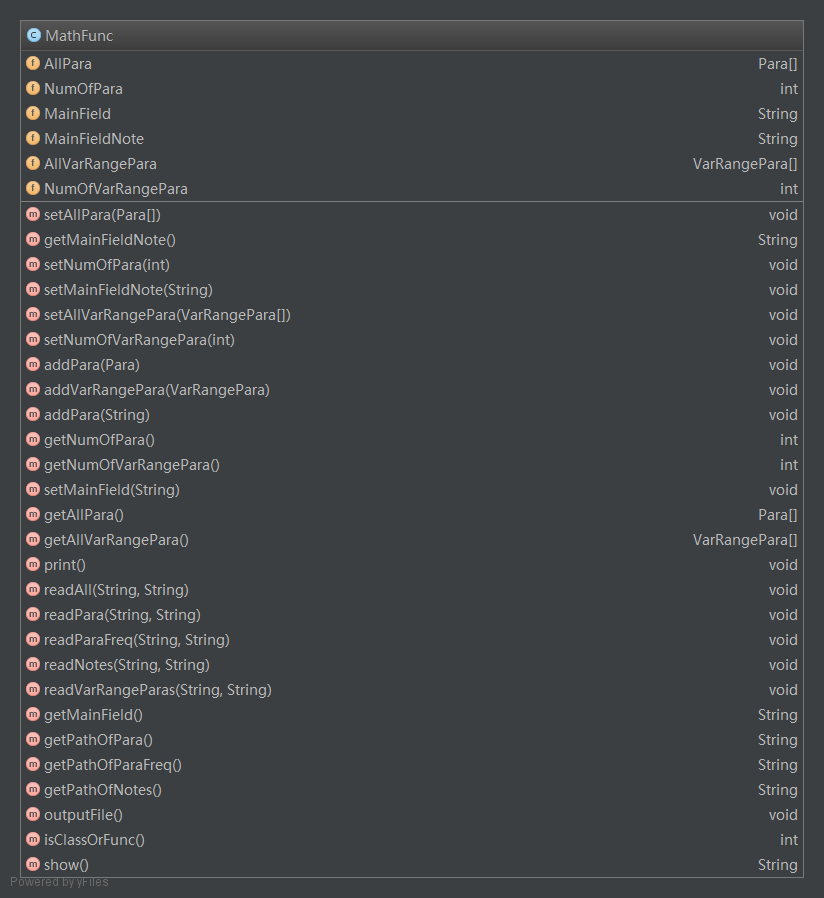
\includegraphics[width=3in]{MathFunc.png}
				\caption{MathFunc类}
				\label{pic:GUIPack}
				\end{minipage}
			\end{figure}

			FuncClass类描述了一个函数类,其下可包含若干个函数类(FuncClass)与函数(MathFunc),函数的方法较多,因此没有显示在图中,主要为获取与设置成员变量值,实现文件读写,添加函数类,添加函数,生成其下所包含对象的树结构等功能。

			MathFunc类描述了一个函数,其下可包含若干个参数,其方法如图所示,主要为获取与设置成员变量值,实现添加参数,文件读写,生成代码等功能。

		% subsection funcclass (end)

		\subsection{Para与VarRangePara类} % (fold)
		\label{sub:para}


			\begin{figure}[!h]
				\begin{minipage}[b]{0.45\textwidth}
				\centering
				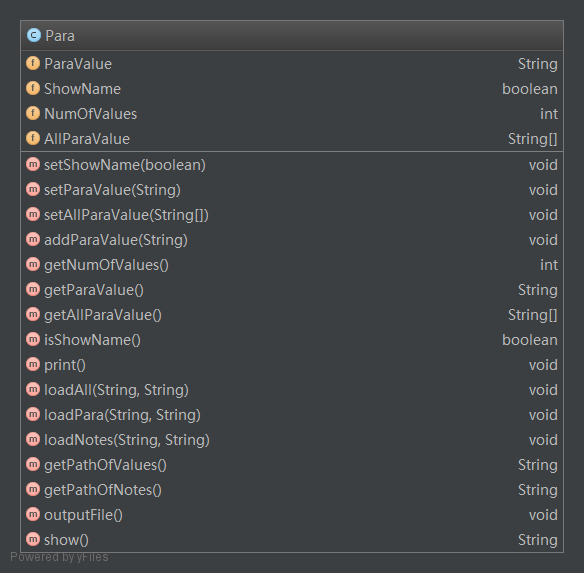
\includegraphics[width=3in]{Para.png}
				\caption{Para类}
				\label{pic:MathPack}
				\end{minipage}%
				\hspace{0.1\textwidth}%
				\begin{minipage}[b]{0.45\textwidth}
				\centering
				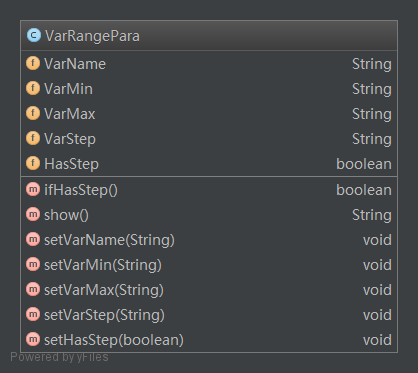
\includegraphics[width=3in]{VarRangePara.png}
				\caption{VarRangePara类}
				\label{pic:GUIPack}
				\end{minipage}
			\end{figure}

			Para类描述了一个Mathematica函数的参数,有参数可取值,参数取值,参数个数,参数是否被使用等成员变量,以及添加参数可取值,获取成员变量值与设置成员变量值,生成代码等方法。

			VarRangePara类描述了一个变量范围类型的Mathematica函数变量,包含L了起点,步长,终点,是否含有步长,参数是否被使用等成员变量,以及获取成员变量值与设置成员变量值,生成代码等方法。

		% subsection para (end)

		
		
	% section 数学相关类 (end)

	\section{用户界面相关类} % (fold)


		\subsection{MainFrame与MainPane类} % (fold)
		\label{sub:mainframe}
			\begin{figure}[!h]
				\begin{minipage}[b]{0.45\textwidth}
				\centering
				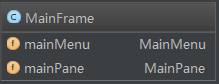
\includegraphics[width=3in]{MainFrame.png}
				\caption{MainFrame类}
				\label{pic:MathPack}
				\end{minipage}%
				\hspace{0.1\textwidth}%
				\begin{minipage}[b]{0.45\textwidth}
				\centering
				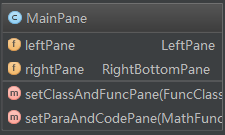
\includegraphics[width=2.5in]{MainPane.png}
				\caption{MainPane类}
				\label{pic:GUIPack}
				\end{minipage}
			\end{figure}
		% subsection mainframe (end)

		MainFrame与MainPane为图形用户界面的两个基础类,MainFrame即为整个用户界面的框架,包含MainPane与MainMenu。而MainPane则为显示所有相关信息的主面板的类,主面板分为左右两个部分,在用户界面设计会有更详细的描述。MainPane有用于在用户进行相应操作后更新面板内容的方法。

		\subsection{RightBottomPane与ParaAndCodePane类} % (fold)
		\label{sub:rightbottompane}

			\begin{figure}[!h]
				\begin{minipage}[b]{0.45\textwidth}
				\centering
				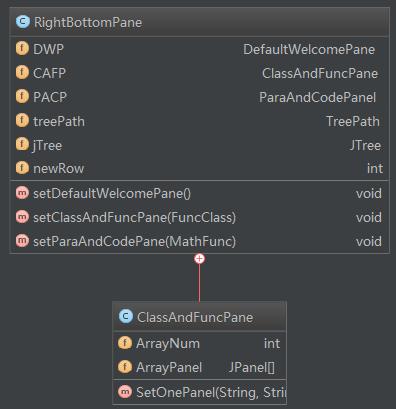
\includegraphics[width=2.5in]{RightBottomPane.png}
				\caption{RightBottomPane类}
				\label{pic:MathPack}
				\end{minipage}%
				\hspace{0.1\textwidth}%
				\begin{minipage}[b]{0.45\textwidth}
				\centering
				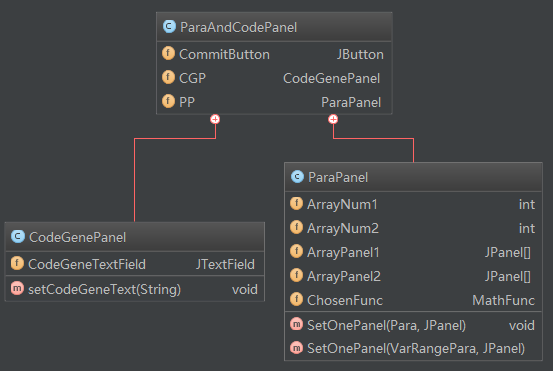
\includegraphics[width=3in]{ParaAndCodePane.png}
				\caption{ParaAndCodePane类}
				\label{pic:GUIPack}
				\end{minipage}
			\end{figure}
			
			RightBottomPane与ParaAndCodePane均为描述主面板右侧子面板的类。

			RightBottomPane类包含了DefaultWelcomePane,ClassAndFuncPane,ParaAndCodePane三个类的对象成员,分别为显示默认欢迎界面,函数类与函数信息界面与函数设置界面的类,且有用于在用户进行相应操作后更新面板内容的方法。

			ParaAndCodePane为显示函数设置界面的类,包含设置部分的子面板与生成代码部分的子面板对应的子类ParaPanel与CodeGenePanel。其中ParaPanel会根据函数参数个数的不同动态生成参数设置部分的子面板,包含对应于Para与VarRangePara两种类型的参数分别生成子面板的成分,最终生成完整的设置部分的子面板。

		% subsection rightbottompane (end)

		\subsection{PopupFrame与PopupSearchFrame} % (fold)
		\label{sub:popupframe}
			
			\begin{figure}[!h]
				\begin{minipage}[b]{0.6\textwidth}
				\centering
				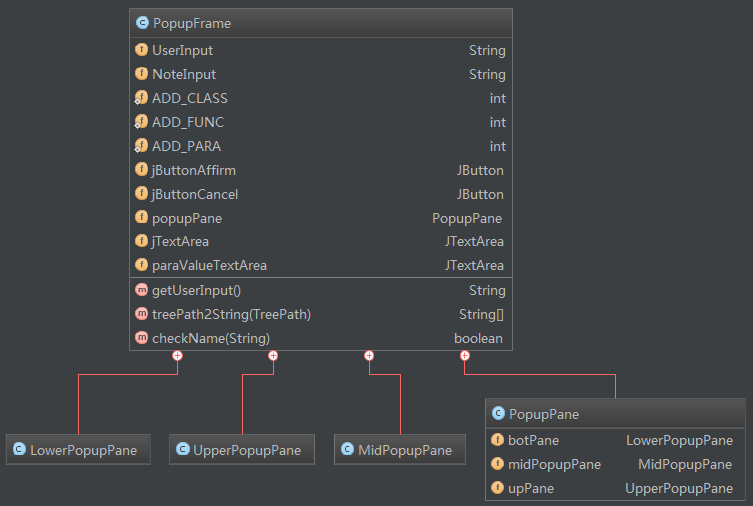
\includegraphics[width=3.7in]{PopupFrame.png}
				\caption{PopupFrame类}
				\label{pic:MathPack}
				\end{minipage}%
				\hspace{0.05\textwidth}%
				\begin{minipage}[b]{0.3\textwidth}
				\centering
				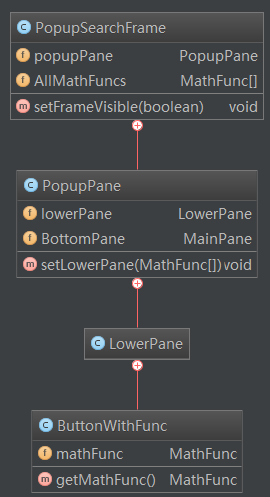
\includegraphics[width=1.7in]{PopupSearchFrame.png}
				\caption{PopupSearchFrame类}
				\label{pic:GUIPack}
				\end{minipage}
			\end{figure}

			PopupFrame与PopupSearchFrame均为实现弹出对话框的类,其中PopupFrame实现添加函数类,添加函数与添加参数三种功能,PopupSearchFrame实现通过函数名称搜索函数的功能。

			PopupFrame的面板由三部分组成,分别对应三个子类。其包含三个静态成员变量以标记被调用时是用于实现添加函数类,添加函数与添加参数三种功能中的哪一种。对于用户的输入,有chechName方法用于判断输入的合理性。

			PopupSearchFrame的面板由两个部分组成,分别为用户输入与搜索结果,包含为实现点击效果的ButtonWithFunc子类。下面板有方法实现用户输入实时变化时的实时更新功能。

		% subsection popupframe (end)

	% section 用户界面相关类 (end)

\chapter{用户界面设计}

	\section{主界面} % (fold)

		\begin{figure}[!h]
			\centering
			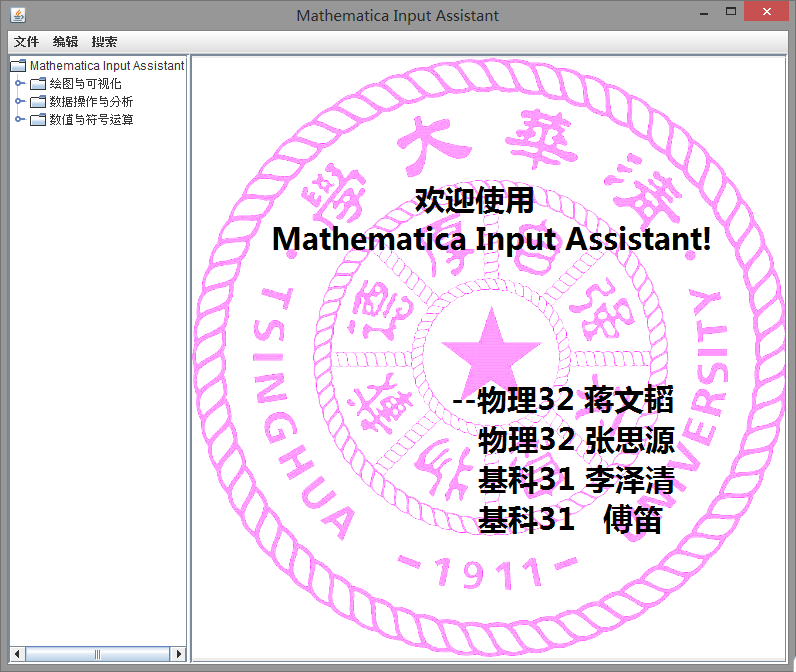
\includegraphics[width=5in]{Welcome.png}
			\caption{主界面效果图}	
		\end{figure}

		主界面如图所示,主要由菜单栏,左侧界面与右侧界面组成。左侧界面为包含所有函数类与函数的树形结构,供用户查找包含其想使用的功能的函数类与函数。右侧界面在未选中任何函数类或函数时为默认的欢迎界面。
		
	% section 主界面 (end)
	\section{菜单栏} % (fold)

		\begin{figure}[!h]
			\begin{minipage}[b]{0.3\textwidth}
			\centering
			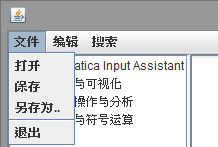
\includegraphics[width=1.7in]{Menu1.png}
			\label{pic:MathPack}
			\end{minipage}%
			\hspace{0.025\textwidth}%
			\begin{minipage}[b]{0.3\textwidth}
			\centering
			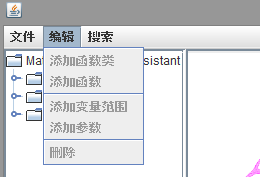
\includegraphics[width=1.7in]{Menu2.png}
			\label{pic:GUIPack}
			\end{minipage}			
			\hspace{0.025\textwidth}%
			\begin{minipage}[b]{0.3\textwidth}
			\centering
			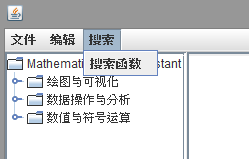
\includegraphics[width=1.7in]{Menu3.png}
			\label{pic:GUIPack}
			\end{minipage}
			\caption{菜单栏效果图}
		\end{figure}

		菜单栏主要由三个子栏组成,如图所示。在未选中任何函数类或函数的情况下时,编辑栏中的选项均为不可用。选中函数类或函数时,启用的选项会相应变化。

	% section 菜单栏 (end)


	\section{左侧界面} % (fold)

		\begin{figure}[!h]
			\begin{minipage}[b]{0.15\textwidth}
			\centering
			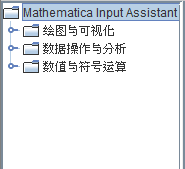
\includegraphics[width=1in]{Left1.png}
			\label{pic:MathPack}
			\end{minipage}%
			\hspace{0.025\textwidth}%
			\begin{minipage}[b]{0.15\textwidth}
			\centering
			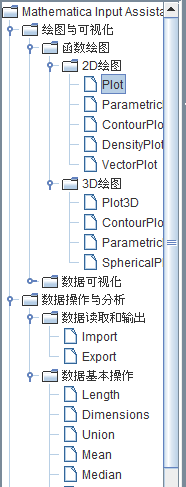
\includegraphics[width=1in]{Left2.png}
			\label{pic:GUIPack}
			\end{minipage}			
			\hspace{0.025\textwidth}%
			\begin{minipage}[b]{0.6\textwidth}
			\centering
			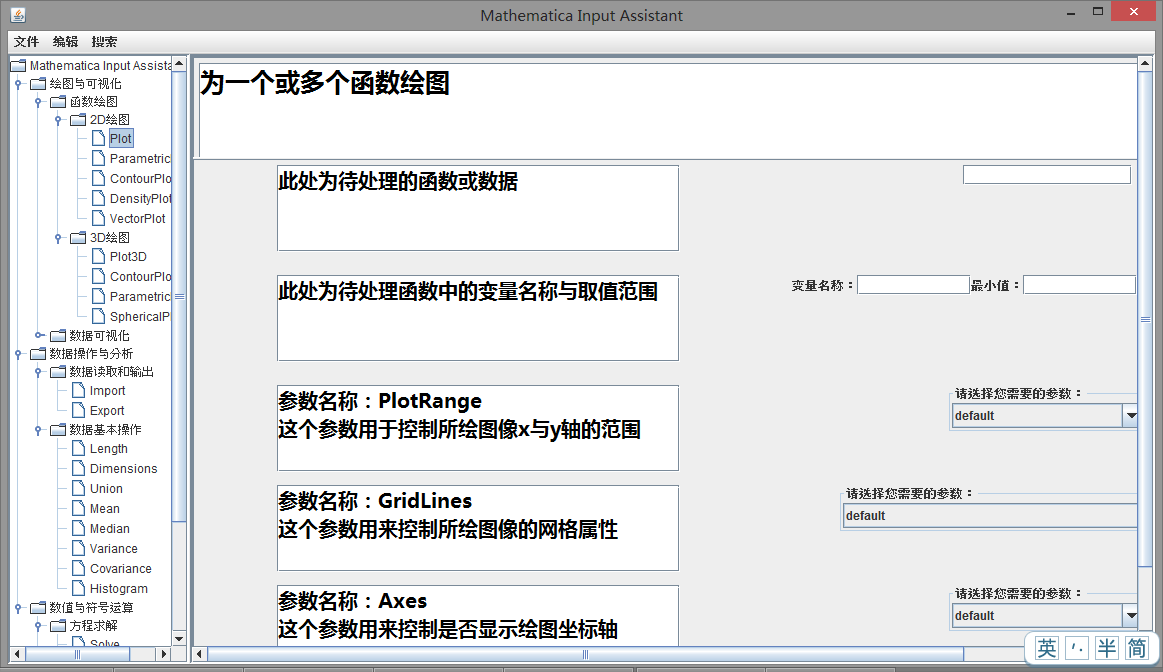
\includegraphics[width=4in]{Left3.png}
			\label{pic:GUIPack}
			\end{minipage}
			\caption{左侧界面效果图}
		\end{figure}

		左侧界面为包含所有函数类与函数的树形结构,供用户查找包含其想使用的功能的函数类与函数。当展开节点较多时,会出现滚动条使用户可以拖动以查看完整的树形结构。当点击相应节点时,右侧界面能够有相应的响应。
		
	% section 左侧界面 (end)

	\section{介绍界面} % (fold)

		\begin{figure}[!h]
			\begin{minipage}[b]{0.45\textwidth}
			\centering
			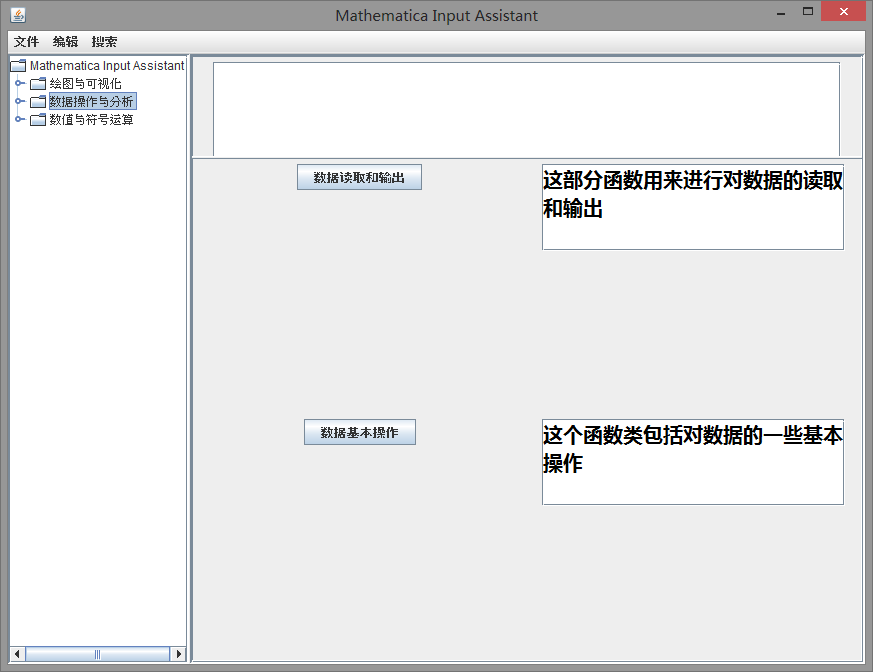
\includegraphics[width=3in]{Right01.png}
			\label{pic:MathPack}
			\end{minipage}%
			\hspace{0.1\textwidth}%
			\begin{minipage}[b]{0.45\textwidth}
			\centering
			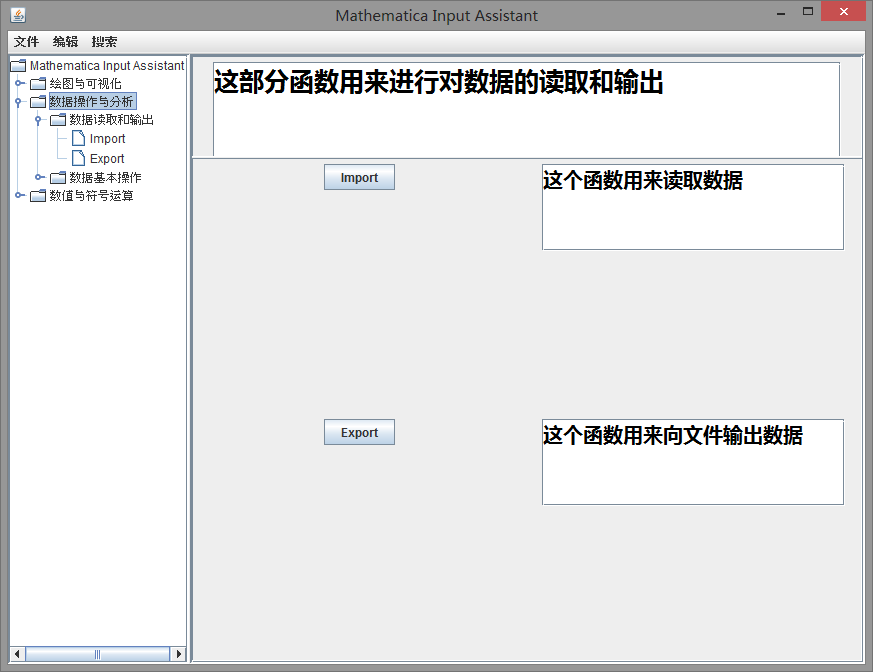
\includegraphics[width=3in]{Right02.png}
			\label{pic:GUIPack}
			\end{minipage}
			\caption{介绍界面效果图}
		\end{figure}

		介绍界面为显示被选中的函数类下的函数类与函数的名称与简介。其中名称对应的按钮可以点击并发生相应跳转。同时,左侧节点的展开情况也会发生相应变化。


		
	% section 介绍界面 (end)

	\section{函数设定界面} % (fold)


		\begin{figure}[!h]
			\begin{minipage}[b]{0.45\textwidth}
			\centering
			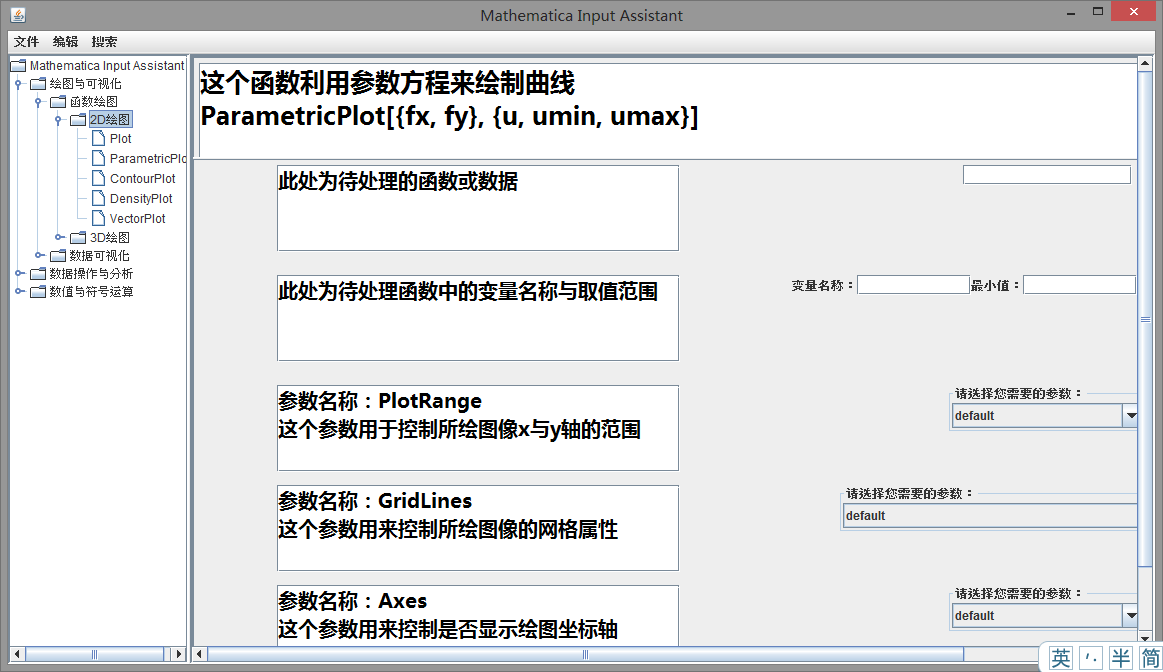
\includegraphics[width=3in]{Right2.png}
			\label{pic:MathPack}
			\end{minipage}%
			\hspace{0.1\textwidth}%
			\begin{minipage}[b]{0.45\textwidth}
			\centering
			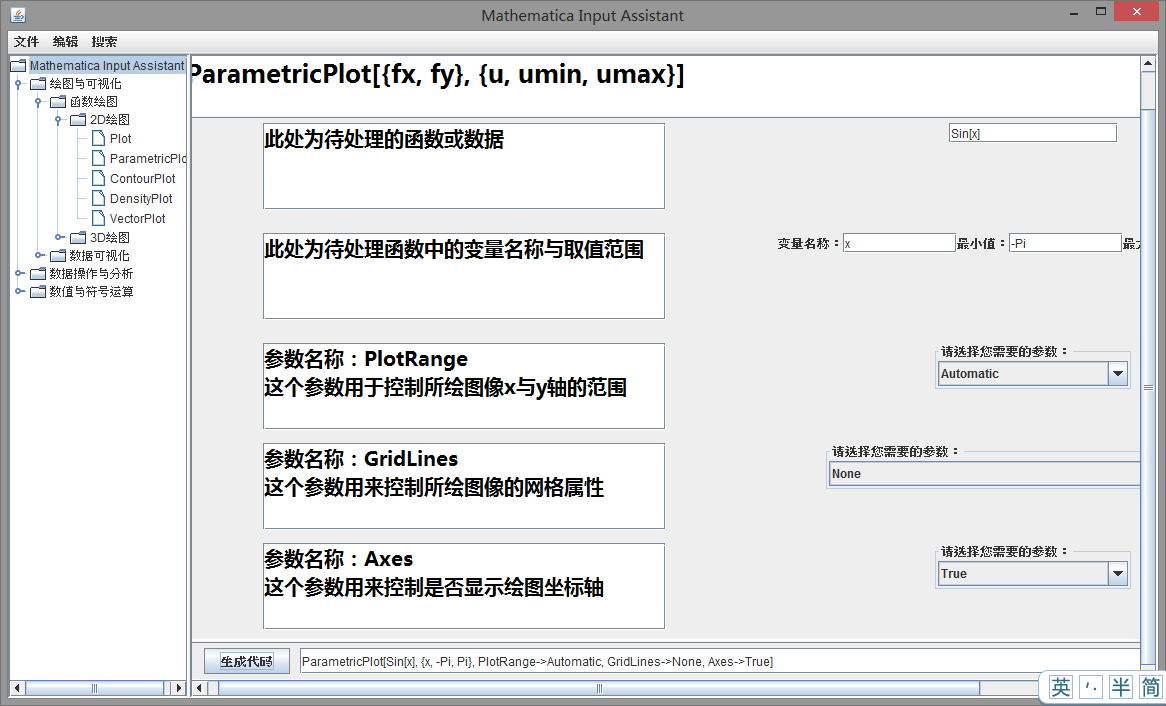
\includegraphics[width=3in]{Right3.png}
			\label{pic:GUIPack}
			\end{minipage}
			\caption{函数设定界面效果图}
		\end{figure}

		函数设定界面可显示出该函数所需的所有参数以及相应说明,供用户设定。当用户设定了所需的参数后,即可通过点击生成代码,生成出可直接拷贝到Mathematica中直接运行的代码,如右图所示。

		
	% section 函数设定界面 (end)

	\section{弹出界面与对话框} % (fold)
		
		\subsection{添加函数类,函数与参数界面} % (fold)

			\begin{figure}[!h]
				\begin{minipage}[b]{0.3\textwidth}
				\centering
				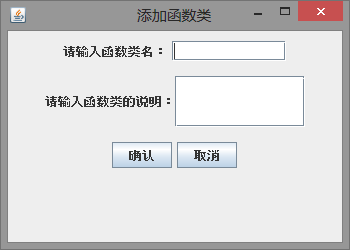
\includegraphics[width=1.7in]{AddFuncClass.png}
				\label{pic:MathPack}
				\end{minipage}%
				\hspace{0.025\textwidth}%
				\begin{minipage}[b]{0.3\textwidth}
				\centering
				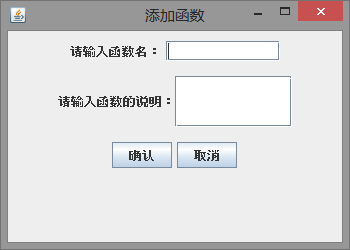
\includegraphics[width=1.7in]{AddMathFunc.png}
				\label{pic:GUIPack}
				\end{minipage}			
				\hspace{0.025\textwidth}%
				\begin{minipage}[b]{0.3\textwidth}
				\centering
				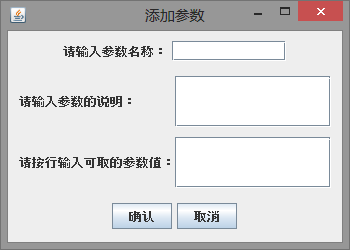
\includegraphics[width=1.7in]{AddPara.png}
				\label{pic:GUIPack}
				\end{minipage}
				\caption{添加功能弹窗效果图}
			\end{figure}

			添加添加函数类,函数与参数的弹出界面如图所示,简洁明了,并且对于函数名会检查用户输入是否合理,否则会弹窗提醒。成功添加后即可在右下界面看到变化。


		% subsection 添加函数类界面 (end)

		\subsection{添加变量对话框,删除对话框与搜索对话框} % (fold)

			\begin{figure}[!h]
				\begin{minipage}[b]{0.3\textwidth}
				\centering
				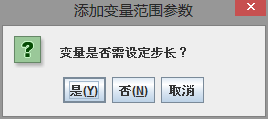
\includegraphics[width=1.7in]{AddVR.png}
				\label{pic:MathPack}
				\end{minipage}%
				\hspace{0.025\textwidth}%
				\begin{minipage}[b]{0.3\textwidth}
				\centering
				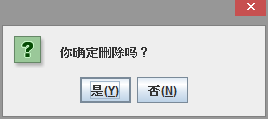
\includegraphics[width=1.7in]{Delete.png}
				\label{pic:GUIPack}
				\end{minipage}			
				\hspace{0.025\textwidth}%
				\begin{minipage}[b]{0.3\textwidth}
				\centering
				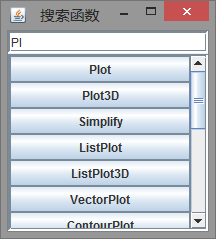
\includegraphics[width=1.7in]{Search.png}
				\label{pic:GUIPack}
				\end{minipage}
				\caption{添加变量,删除与搜索对话框效果图}
			\end{figure}

			添加变量,删除与搜索对话框如图所示。其中搜索对话框的搜索结果会随用户输入而实时变化,搜索结果较多时会出现滚动条。点击某一个搜索结果,搜索框即会消失,并且主面板的右侧将跳转至选中的搜索结果所对应的函数的设置界面。
			
		% subsection 添加变量对话框 (end)

	% section 弹出界面 (end)

	\section{主要设计原则} % (fold)

	\begin{itemize}
		\item 界面组成简介,组件逻辑与依赖关系清晰
		\item 使用户能够根据自己需求依次寻找到对应的函数
		\item 用户可实现的操作多样且人性化
		\item 所有需要用户操作的组件均设置说明
		\item 注意避免显示区域有限导致部分组件不可见的问题
	\end{itemize}
	
	% section 主要设计原则 (end)

\chapter{反思} % (fold)
\label{cha:}
	经过设计与实际软件的编写与实现后,我们发现了设计中的一些问题并进行了反思,主要有
	\begin{itemize}
		\item 类结构设计有待改进,如文件的读写部分应与MathFunc包中的类分离开
		\item GUI中用户响应部分的处理有待改进,虽然实现了所设计的功能但因设计不够详细而导致实现方法不统一,可能导致维护与修改的不便
	\end{itemize}
% chapter  (end)

\end{document}